\documentclass{article}
\usepackage{tikz}
\usepackage{hyperref}
\usepackage{amsmath}
\usepackage{mathtools}
\usepackage{float}
\usepackage{xcolor}
\usepackage[a4paper]{geometry}
\usepackage[textsize=small,textwidth=100]{todonotes}

\usetikzlibrary{positioning,arrows,backgrounds}
\usepgflibrary{shapes.geometric}

\tikzset{%
vertex/.style={draw,fill,circle,minimum size=5pt,inner sep=1pt},
hyperedge/.style={draw,rectangle},
tentacle/.style={pos=0.2,auto,font=\tiny,minimum size=1pt,inner sep=1pt},
flowcond/.style={diamond,minimum size=40pt,draw},
tinylabel/.style={font=\tiny,inner sep=1pt,right=0mm of #1},
every label/.style={font=\tiny,inner sep=1pt,label position=right},
blank/.style={inner sep=0,minimum size=0}
}

\newcommand{\code}[1]{\texttt{#1}}

\begin{document}
\title{Generating Random Graphs with Graph Grammars}
\author{Jake Coxon}
\maketitle

\tableofcontents

\section{Introduction}
Introduction should go here

\section{Literature Review}

\subsection{Graphs}
  \begin{figure}
  \centering
  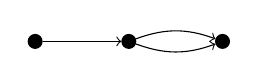
\begin{tikzpicture}
    \node[vertex] (a)    {};
    \node[vertex] (b) [right=of a]  {};
    \node[vertex] (c) [right=of b]  {};
    \path[->] (a) edge (b)
              (b) edge [bend left=20] (c) 
                  edge [bend right=20] (c);
  \end{tikzpicture}
  \caption{A directed multigraph}
\end{figure}

  A graph is a finite set of points known as vertices that are interconnected by a set of lines (edges). Edges connect exactly two vertices that shows a relation.

  A label alphabet $L = \langle L_v, L_e \rangle$ consists of a set $L_v$ of node labels and a set $L_e$ of edge labels.

  A graph over $L$ is a system $G = \langle V_G, E_G, s_G, t_G, l_G, m_G \rangle$ where $V_G$ and $E_G$ are finite sets of vertices and edges respectively. $s_G, t_G : E_G \to V_G$ are functions assigning a source and a target to each edge. $l_G : V_G \to L_V$ and $m_G : E_G \to L_E$ are functions assigning a label to each node and edge\cite{Detlef1}.

  Different types of graphs exist pertaining to different problems. Graph edges can be weighted and/or directed and vertices can be labelled. Graphs can allow edges to be looped where both endpoints point to the same vertex. Multi-graphs are graphs where multiple edges can exist between a pair a vertices.

\subsection{Hypergraphs}
  \begin{figure}
  \centering
  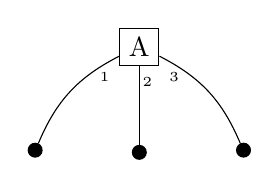
\begin{tikzpicture}

    \node[hyperedge] (hyp)    {A};
    \node[vertex] (a) [below left=of hyp] {};
    \node[vertex] (b) [below=of hyp]  {};
    \node[vertex] (c) [below right=of hyp] {};


    \path[-] (hyp) edge [bend right=20] node[tentacle]{$1$} (a)
                   edge [-] node[tentacle]{$2$} (b)
                   edge [bend left=20] node[tentacle,auto=right]{$3$} (c);
  \end{tikzpicture}
  \caption{A hypergraph with a hyperedge labeled $A$}
\end{figure}

  A generalised version of graphs are hypergraphs. Within a hypergraph, a hyperedge is similar to an edge except it is connected to any number of vertices. The connections between a hyperedge and a vertex is known as `tentacles' and the number of the tentacles a hyperedge has is known as its type. A graph is a specialised version of a hypergraph where all hyperedges has type of $2$.

  An alphabet $C$ is a fixed set containing labels. A hypergraph over $C$ is a system $F = \langle V_F, E_F, att_F, lbl_F \rangle$ where $V_F$ and $E_F$ are finite sets of vertices and edges the same as graphs. $att_F : E_F \to V_F*$ is a mapping assigning a sequence of `attachment nodes' to each edge $e \in E_F$ and $lbl_F$ is a mapping that labels hyperedges. 

  The $type(E)$ of an edge is the number of vertices that a hyperedge attaches to. A tentacle is an object used to describe the attachment of a hyperedge to a vertex.

  %\todo{C???}

  \begin{figure}[!h]
  \centering
  \begin{tikzpicture}
    \node[] (a)    {};
    \node[flowcond] (cond) [below=of a]  {};
    \node[] (b) [below left=of cond]  {};
    \node[] (c) [below right=of cond] {};

    \path[<-] (cond) edge (a);
    \draw[->] (cond) -| (b);
    \draw[->] (cond) -| (c);
  \end{tikzpicture}
  \caption{Hyperedges can be used to model flowcharts}
\end{figure}

\subsection{Random Graph Generation}
  Random graph generators are systems to generate a single or set of graphs based on some non-deterministic rules. This can be used as test data for programs for testing speed and memory. It can also be used for verifying whether a property is true for a range of graphs in a range or seeing how \emph{often} a property is true for a range of graphs.

  There are two methods for random graph generation described in \cite{Skiena}:

  Random Edge Generation---Every pair of vertices is listed and a coin is flipped to decide whether an edge is produced between them.

  Random Edge Selection---For a desired number of edges $m$, it selects $m$ distinct edges at random.

  Both of these methods have their limitations. With these methods you cannot enforce the structure of the graph, for instance it is impossible to generate multi-graphs and it is not likely to generate a cyclic graph. For the purposes of testing algorithms, these methods aren't good enough, you cannot test an algorithm that only accepts trees unless you can generate only trees.

  \subsubsection{Standford GraphBase}
    The Stanford GraphBase is a collection of programs written by Donald Knuth. Its main purpose is to generate and examine graphs but can also be used as a library to write ones own programs. 

    The programs are written in a language called CWEB which is a combination of \TeX and the C programming language but a person can just as well write a program in C and include the GraphBase library. 

    In GraphBase, graphs are represented by the structures \code{Graph}, \code{Vertex} and \code{Arc}. A Graph ponter $g$ refers to a single graph and $g$ has multiple fields and $g \to n$ is the number of vertices in this graph. $g \to vertices$ an array of all vertices so $g \to vertices[k]$ points to the $k^{th}$ vertex.

    Directed edges between vertices are specified by \code{Arc}s. The head of the linked list contain all arcs for a vertex is stored in $v \to arcs$. To represent undirected edges, two arcs are required. 

    To generate a random graph, the function \code{random\_graph} can be used which generates a random graph based on a number of parameters:

    \begin{itemize}
    \item \code{multi}---whether the graph is permitted to have duplicate arcs eg. a multigraph.
    \item \code{self}---whether the graph can have self-loops.
    \item \code{directed}---if the graph is directed or not.
    \item \code{dist\_from} and \code{dist\_to}---the probability distributions of arcs to vertices.
    \item \code{min\_len} and \code{max\_len}---the arc lengths will be uniformly distributed between these two values.
    \end{itemize}

    The arrays \code{dist\_from} and \code{dist\_to} are used to control the discrete distribution of the arcs. The probabilities are scaled so the sum of the array is $1$. For example, to define the probability that $v_k$ is twice as likely as $v_{k+1}$ to be the source of an arc, \code{dist\_from} should equal \code{\{...,16,8,4,2,1\}}

    The function will return a \code{Graph} structure so in order to output, analyse or perform any validation on the graph, the user of this library must do some extra work himself.

  \subsubsection{Mathematica}
    Wolfram Mathematica is a powerful integrated environment which allows the user to input an expression language within the program. Previously, the package Combinatorica\footnote{http://www.cs.sunysb.edu/~skiena/combinatorica/} was needed to provide graph theory functions however, Mathematica version 8 added most of these functions natively.

    The programming language in Mathematica enables the user to build expressions and functions. user inputs a command as text and the output of the command is written below. The command \code{Sin[3.4]} will output \code{-0.255541} to the screen.

    The basic function to generate a random graph is \code{RandomGraph[gdist, n]} which generates $n$ graphs with the graph distribution $gdist$. The distribution function \code{BernoulliGraphDistribution} provides the random edge generation method. In the command \code{RandomGraph[BernoulliGraphDistribution[6, 0.5], 3]} we request six vertices and $50\%$ probability that an edge occurs between them. We also request that we want three graphs.

    \begin{figure}[htb]
\centering
\setlength\fboxsep{0pt}
\setlength\fboxrule{0.5pt}
\fcolorbox{lightgray}{white}{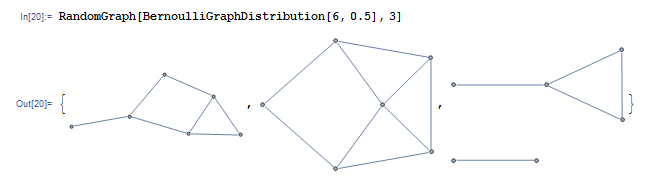
\includegraphics[width=\textwidth]{figures/mathematica-random.png}}
\caption{Mathematica function to generate three graphs}
\end{figure}

    %\todo{Directed graphs, different types of graphs}

    A list of relevent graph distributions is as follows.

    \begin{itemize}
    \item
    \code{BernoulliGraphDistribution[n, p]} generates $n$ vertices and a $p$ chance of an edge occuring between them. This is the random edge generation method decribed above where a fixed amount of vertices will be generated and every pair of vertices will have a probability of an edge occuring between them.

    \item 
    \code{UniformGraphDistribution[n, m]} generates a uniform graph distribution on $n$ vertices and $m$ edges. This distribution is equivilent to the random edge selection method above where there are a fixed number of vertices and edges but the positions of the edges are random generated.

    \item 
    \code{BarabasiAlbertGraphDistribution[n, k]} generates $n$ vertices where a new vertex with $k$ edges is added at each step. This distribution will force each vertex to have at least $k$ edges attached to it.

    \item
    \code{PriceGraphDistribution[n, k, a]} generates a graph with a de Solla Price distribution which is a distribution that gives edges a preferential attachment to vertices.

    \item
    \code{DegreeGraphDistribution[dlist]} generates a graph where $\mathrm{vertex}_i$ has degree $\mathrm{dlist}_i$.
    \end{itemize}

    Additionally the user can use the progamming language to programatically generate a graph based on his own method. There exists functions \code{EdgeAdd} and \code{VertexAdd} which can be combined with some random functions. In the next example, \code{StarGraph[n]} is used which constructs a graph with $n$ vertices with one vertex connected to all others. Next an edge is added onto this graph between $v_2$ and $v_r$ where $v_i$ is vertex $i$ and $r$ is a random number in the range $\{0,...,10\}$.

    \begin{figure}[htb]
\centering
\setlength\fboxsep{0pt}
\setlength\fboxrule{0.5pt}
\fcolorbox{lightgray}{white}{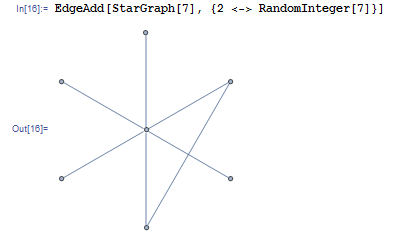
\includegraphics[scale=0.8]{figures/mathematica-star.png}}
\caption{Mathematica function to generate a star}
\end{figure}

    This shows that Mathematica gives the user a powerful set of tools and multiple methods of generating random graphs. However there is no general solution for generating random graphs, the user must learn the programming language and must have a specific algorithm in mind. For anything more advanced than adding specific edges or nodes, the code can get very complex.

    The output graph will be immediately shown to the user and more processing can be done on it. Additionally the data of this graph can be exported in a number of largely used formats including \emph{GraphML}, \emph{GXL}, \emph{Graph6}, \emph{DOT}. Furthermore, the generated image of the graph can be saved for the user to use in documents.

\subsection{Hypergraph Languages}
  \subsubsection{Hyperedge Replacement}

    It is possible to construct new hypergraphs by the replacement of a hyperedge by a new hypergraph to yield a new hypergraph. A hyperedge $e$ in a hypergraph $H$ may be replaced with another hypergraph $R$. An sequence of external nodes $ext$ in $R$ is needed where each node in $ext$ corresponds to an attachment node of $e$.

    A replacement happens by first removing the hyperedge $e$, then adding the hypergraph $R$ excluding external nodes. Then for each hyperedge in $R$ that points to an external node, the tentacle must now point to the corresponding attachment nodes of $e$.

    The replacement of hyperedge $e$ in a hypergraph $H$ with the a hypergraph $R$ is denoted by $H[e/R]$. 

    The definition of hyperedge replacement is as follows:
    \begin{align*}
    V_X &= V_H + (V_R - ext) \\
    E_X &= (E_H - e) + E_R \\
    lbl_X &= lbl_H \cup lbl_R \\
    att_X(e) &= \{handover_e(x_1),...,handover_e(x_n)\} & \text{for all $e \in E_X$ and where $att_H(e) = x_1...x_n$}
    \end{align*}
    Where $handover_e : V_X \to V_X$ is defined by
    \begin{align*}
    handover_e(x_i) &= \begin{dcases*}
    a_i & if $x_i \in ext$ and where $att_H(e) = a_1...a_n$ \\
    x_i & otherwise
    \end{dcases*}
    \end{align*}

    We can see an example of hyperedge replacement here.
    
    \begin{figure}[H]
  \centering
  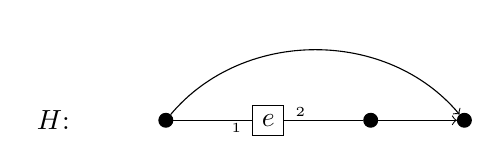
\begin{tikzpicture}

    \node (lbl) {$H$:};
    \node[vertex,right=of lbl] (a) {};
    \node[hyperedge] (hyp) [right=of a] {$e$};
    \node[vertex] (b) [right=of hyp] {};
    \node[vertex] (c) [right=of b] {};


    \path[->] (a) edge [bend left=50] (c)
              (b) edge (c);

    \path[-] (hyp) edge node[tentacle]{$1$} (a)
                   edge node[tentacle]{$2$} (b);

  \end{tikzpicture} \\[0.5cm]
  
  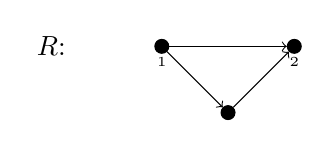
\begin{tikzpicture}

    \node (lbl) {$R$:};
    \node[vertex] (a) [right=of lbl] {} node[below=0mm of a,font=\tiny,inner sep=1pt]{1};
    \node[vertex] (b) [below right=1cm of a] {};
    \node[vertex] (c) [above right=1cm of b] {} node[below=0mm of c,font=\tiny,inner sep=1pt]{2};

    \path[->] (a) edge (b)
                  edge (c)
              (b) edge (c);
  \end{tikzpicture} \\[0.5cm]
  
  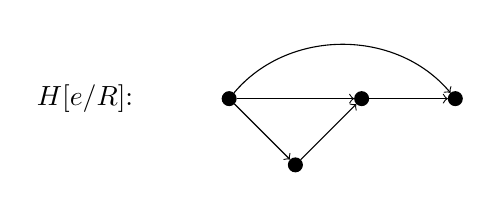
\begin{tikzpicture}

    \node (lbl) {$H[e/R]$:};
    \node[vertex,right=of lbl] (a) {};
    \node[vertex] (b) [below right=1cm of a] {};
    \node[vertex] (c) [above right=1cm of b] {};
    \node[vertex] (d) [right=of c] {};

    \path[->] (a) edge [bend left=50] (d)
                  edge (b)
                  edge (c)
              (b) edge (c)
              (c) edge (d);

  \end{tikzpicture}
  \caption{Hyperedge replacement}
\end{figure}

    A couple of properties can be observed in hyperedge replacement. Firstly, the sequentialization and parallelization property. Given two different replacements, the result will be equivilent whether the replacements happen one after another or simultaneously.

    \begin{equation}
    H[e_1/H_1,...e_n/H_n] = H[e_1/H_1]...[e_n/H_n]
    \end{equation}

    Secondly the replacement is confluent, this means hyperedges in a hypergraph can be replaced in any order without affecting the result.

    \begin{equation}
    H[e_1/H_1][e_2/H_2] = H[e_2/H_2][e_1/H_1]
    \end{equation}

    Finally we know the replacement is associative. If a hyperedge is replaced and then a part of the new hypergraph is replaced, this is equivilent to replacing the second hyperedge and then replacing the first hyperedge with the result.

    \begin{equation}
    H[e_1/H_1][e_2/H_2] = H[e_1/H_1 [e_2/H_2]]
    \end{equation}

  \subsubsection{Hyperedge Replacement Grammars}

    Hypergraphs can be generated using productions based on hyperedge replacement. A production is $p = \langle x \to R, ext \rangle$ where $x$ is a non-terminal so let $H$, $H'$ be hypergraphs and let $e \in E_H$ such that $l_{H}(e) = x$. Then $H$ directly derives $H'$ by $p$ applied to $e$ if $H'$ is equivilent to $H[e / R]$. This can be written $H \underset{p}{\Rightarrow} H'$.

    If we are given a production:
    \begin{figure}[H]
  \centering
  
  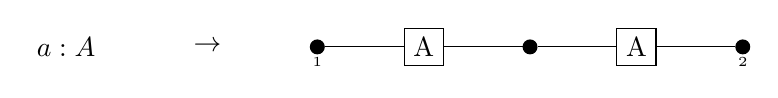
\begin{tikzpicture}

    \node[] (lbl) [] {$a: A$};


    \node[] (arrow1) [right=of lbl] {$\to$};


    \node[vertex] (a) [right=of arrow1] {} node[below=0mm of a,font=\tiny,inner sep=1pt]{1};
    \node[hyperedge] (hyp1) [right=of a] {A};
    \node[vertex] (b) [right=of hyp1] {};
    \node[hyperedge] (hyp2) [right=of b] {A};
    \node[vertex] (c) [right=of hyp2] {} node[below=0mm of c,font=\tiny,inner sep=1pt]{2};

    \path[-] (hyp1) edge node[tentacle]{} (a)
                   edge node[tentacle]{} (b);

    \path[-] (hyp2) edge node[tentacle]{} (b)
                   edge node[tentacle]{} (c);

    %\node[vertex] (a) [right=of arrow1] {} node[below=0mm of a,font=\tiny,inner sep=1pt]{1};
    %\node[vertex] (b) [below right=1cm of a] {};
    %\node[vertex] (c) [above right=1cm of b] {} node[below=0mm of c,font=\tiny,inner sep=1pt]{2};

    %\path[->] (a) edge (b)
    %              edge (c)
    %          (b) edge (c);
  \end{tikzpicture}
  
\end{figure}

    Then it follows:
    \begin{figure}[H]
  \centering
  
  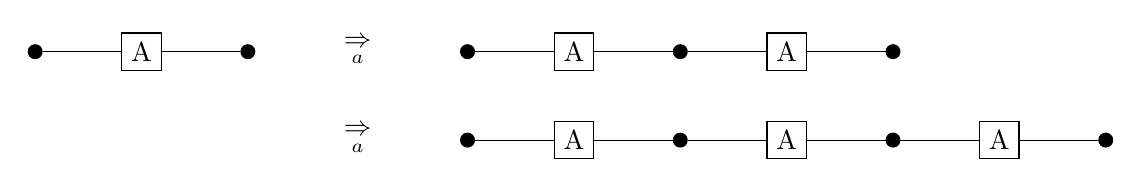
\begin{tikzpicture}

    \node[vertex] (a) [] {};
    \node[hyperedge] (hyp1) [right=of a] {A};
    \node[vertex] (b) [right=of hyp1] {};

    \path[-] (hyp1) edge node[tentacle]{} (a)
                   edge node[tentacle]{} (b);

    \node[] (arrow1) [right=of b] {$\underset{a}{\Rightarrow}$};

    \node[vertex] (a) [right=of arrow1] {};
    \node[hyperedge] (hyp1) [right=of a] {A};
    \node[vertex] (b) [right=of hyp1] {};
    \node[hyperedge] (hyp2) [right=of b] {A};
    \node[vertex] (c) [right=of hyp2] {};

    \path[-] (hyp1) edge node[tentacle]{} (a)
                   edge node[tentacle]{} (b);

    \path[-] (hyp2) edge node[tentacle]{} (b)
                   edge node[tentacle]{} (c);

   \node[] (arrow2) [below=0.5cm of arrow1] {$\underset{a}{\Rightarrow}$};

    \node[vertex] (a) [right=of arrow2] {};
    \node[hyperedge] (hyp1) [right=of a] {A};
    \node[vertex] (b) [right=of hyp1] {};
    \node[hyperedge] (hyp2) [right=of b] {A};
    \node[vertex] (c) [right=of hyp2] {};
    \node[hyperedge] (hyp3) [right=of c] {A};
    \node[vertex] (d) [right=of hyp3] {};

    \path[-] (hyp1) edge node[tentacle]{} (a)
                   edge node[tentacle]{} (b);

    \path[-] (hyp2) edge node[tentacle]{} (b)
                   edge node[tentacle]{} (c);

    \path[-] (hyp3) edge node[tentacle]{} (c)
                   edge node[tentacle]{} (d);

  \end{tikzpicture}
  
\end{figure}

    A hyperedge replacement grammar (HR grammar) is a system for generating a hypergraph language through a set of derivations. It is similar to other language generation concepts in computer science.

    A HR grammar can be defined as $G = \langle N, T, P, S \rangle$ where $N$ is a set of non-terminals, $T$ is a set of terminals disjoint with $N$, $S$ is the start graph. $P$ is a set of productions which are in the form of $\langle x \to R, ext \rangle$ where $x \in N$, $R$ is a hypergraph and $ext$ is the sequence of external nodes in $R$.

    The language of a control flow graph can be generated with the following
    \tikzset{
    every node/.style={scale=0.8,node distance=0.8cm and 0.6cm,anchor=center},
    seperator/.style={color=lightgray},
    aligned/.style={
      to path={
        (\tikztostart) -| (\tikztotarget)
        \tikztonodes
      }
    },
    bent left down/.style={
      to path={
        -- +(-0.5cm,0) .. controls +(-0.5,-0.5) and +(-0.5,0.2) ..  (\tikztotarget) \tikztonodes
      }},
    bent right down/.style={
      to path={
        -- +(0.5cm,0) .. controls +(0.5,-0.5) and +(0.5,0.2) ..  (\tikztotarget) \tikztonodes
      }},
    bent left up/.style={
      to path={
        -- +(-0.5cm,0) .. controls +(-0.5,0.5) and +(-0.5,-0.2) ..  (\tikztotarget) \tikztonodes
      }},
    bent right up/.style={
      to path={
        -- +(0.5cm,0) .. controls +(0.5,0.5) and +(0.5,-0.2) ..  (\tikztotarget) \tikztonodes
      }},
    bent right up big/.style={
      to path={
        -- +(0.5cm,0) .. controls +(0.5,1) and +(1,-0.2) ..  (\tikztotarget) \tikztonodes
      }},
    bent left up big/.style={
      to path={
        -- +(-0.5cm,0) .. controls +(-0.5,1) and +(-1,-0.2) ..  (\tikztotarget) \tikztonodes
      }},
    dhyperedge/.style={hyperedge,diamond},
    dbelow/.style={below=#1.center,anchor=center},
    dbelow2/.style={below=1.6 #1.center,anchor=center},
    dbelow3/.style={below=2.4 #1.center,anchor=center},
    dbelow4/.style={below=3.2 #1.center,anchor=center},
    dbelow left/.style={below left=#1.center,anchor=center},
    dbelow left2/.style={below left=1.6 and 0.6 #1.center,anchor=center},
    dbelow left3/.style={below left=2.4 and 0.6 #1.center,anchor=center},
    dbelow right/.style={below right=#1.center,anchor=center},
    dbelow right2/.style={below right=1.6 and 0.6 #1.center,anchor=center},
    dbelow right3/.style={below right=2.4 and 0.6 #1.center,anchor=center},
  }

\begin{figure}[H]
  \centering
  

  

  \begin{tikzpicture}[scale=0.5,node distance=0.5cm]

    \matrix[column sep=0.5cm]
    {
    \node (lbl) {$C ::= $};

    &

    \node[vertex]     (a)    [label=1] {};
    \node[hyperedge]  (hyp1) [dbelow=of a] {$C$};
    \node[vertex]     (b)    [dbelow=of hyp1] {};
    \node[hyperedge]  (hyp2) [dbelow=of b] {$C$};
    \node[vertex]     (c)    [dbelow=of hyp2,label=2] {} ;

    \path[-] (hyp1) edge node[tentacle]{$1$} (a)
                    edge node[tentacle]{$2$} (b)
             (hyp2) edge node[tentacle]{$1$} (b)
                    edge node[tentacle]{$2$} (c);

    &
      \draw[seperator] (0,0) -- (0,-3.2);
    &

    \node[vertex]     (a)    [label=1] {};
    \node[dhyperedge] (hyp1) [dbelow2=of a] {$D$};
    \node[vertex]     (b)    [dbelow2=of hyp1,label=2] {};

    \path[-] (hyp1) edge node[tentacle]{$1$} (a)
                    edge[bent left down] node[tentacle]{$2$} (b) 
                    edge[bent right down] node[tentacle]{$3$} (b);


    &
      \draw[seperator] (0,0) -- (0,-3.2);
    &
    
    \node[vertex]     (a)    [label=1] {};
    \node[dhyperedge] (hyp1) [dbelow2=of a] {$D$};
    \node[vertex]     (b)    [dbelow2=of hyp1,label=2] {};

    \path[-] (hyp1) edge node[tentacle]{$1$} (a)
                    edge[bent left up] node[tentacle]{$2$} (a) 
                    edge[bent right down] node[tentacle]{$3$} (b);

    &
      \draw[seperator] (0,0) -- (0,-3.2);
    &
    
    \node[vertex]     (a)    [label=1] {};
    \node[dhyperedge] (hyp1) [dbelow2=of a] {$D$};
    \node[vertex]     (b)    [dbelow2=of hyp1,label=2] {};

    \path[-] (hyp1) edge node[tentacle] {$1$} (a)
                    edge[bent left down] node[tentacle] {$2$} (b) 
                    edge[bent right up] node[tentacle] {$3$} (a);
    
    &
      \draw[seperator] (0,0) -- (0,-3.2);
    &

    \node[vertex]     (a)    [label=1] {};
    \node[hyperedge]  (hyp1) [dbelow2=of a] {$c$};
    \node[vertex]     (b)    [dbelow2=of hyp1,label=2] {};

    \path[-] (hyp1) edge node[tentacle]{$1$} (a)
                    edge node[tentacle]{$2$} (b);
    \\
    };
  \end{tikzpicture} \\[1cm]

  \begin{tikzpicture}[scale=0.1,node distance=0.5cm]
    \matrix[column sep=0.5cm,row sep=1cm]
    {

    \node (lbl) {$D ::= $};

    &

    \node[vertex]     (a)    [label=1] {};
    \node[dhyperedge] (hyp1) [dbelow=of a] {$D$};
    \node[vertex]     (b)    [dbelow right=of hyp1] {};
    \node[hyperedge]  (hyp2) [dbelow=of b] {$C$};
    \node[vertex]     (d)    [dbelow=of hyp2,label=3] {};
    \node[vertex]     (c)    [dbelow left3=of hyp1,label=2] {};

    \path[-] (hyp1) edge node[tentacle]{$1$} (a)
                    edge[aligned] node[tentacle]{$2$} (c) 
                    edge[aligned] node[tentacle]{$3$} (b)
             (hyp2) edge node[tentacle]{$1$} (b)
                    edge node[tentacle]{$2$} (d);


    &
      \draw[seperator] (0,0) -- (0,-3.2);
    &

    \node[vertex]     (a)    [label=1] {};
    \node[dhyperedge] (hyp1) [dbelow=of a] {$D$};
    \node[vertex]     (b)    [dbelow left=of hyp1] {};
    \node[hyperedge]  (hyp2) [dbelow=of b] {$C$};
    \node[vertex]     (c)    [dbelow=of hyp2,label=2] {};
    \node[vertex]     (d)    [dbelow right3=of hyp1,label=3] {};

    \path[-] (hyp1) edge node[tentacle]{$1$} (a)
                    edge[aligned] node[tentacle]{$2$} (b)
                    edge[aligned] node[tentacle]{$3$} (d)
             (hyp2) edge node[tentacle]{$1$} (b)
                    edge node[tentacle]{$2$} (c);

    &
      \draw[seperator] (0,0) -- (0,-3.2);
    &

    \node[vertex]     (a)    [label=1] {};
    \node[dhyperedge] (hyp1) [dbelow=of a] {$D$};
    \node[vertex]     (b)    [dbelow left=of hyp1] {};
    \node[dhyperedge] (hyp2) [dbelow=of b] {$D$};
    \node[vertex]     (c)    [dbelow right=of hyp2,label=2] {};
    \node[vertex]     (d)    [dbelow right3=of hyp1,label=3] {};

    \path[-] (hyp1) edge node[tentacle]{$1$} (a)
                    edge[aligned] node[tentacle]{$2$} (b) 
                    edge[aligned] node[tentacle]{$3$} (d)
             (hyp2) edge node[tentacle]{$1$} (b)
                    edge[bent left up big] node[tentacle]{$2$} (a)
                    edge[aligned] node[tentacle]{$3$} (c);
    
    &
      \draw[seperator] (0,0) -- (0,-3.2);
    &

    \node[vertex]     (a)    [label=1] {};
    \node[dhyperedge] (hyp1) [dbelow=of a] {$D$};
    \node[vertex]     (b)    [dbelow right=of hyp1] {};
    \node[dhyperedge] (hyp2) [dbelow=of b] {$D$};
    \node[vertex]     (c)    [dbelow left3=of hyp1,label=2] {};
    \node[vertex]     (d)    [dbelow left=of hyp2,label=3] {};

    \path[-] (hyp1) edge node[tentacle]{$1$} (a)
                    edge[aligned] node[tentacle]{$2$} (c) 
                    edge[aligned] node[tentacle]{$3$} (b)
             (hyp2) edge node[tentacle]{$1$} (b)
                    edge[aligned] node[tentacle]{$2$} (d)
                    edge[bent right up big] node[tentacle]{$3$} (a);

    &
      \draw[seperator] (0,0) -- (0,-3.2);
    

    \\

    &
    
    \node[vertex]     (a)    [label=1] {};
    \node[dhyperedge] (hyp1) [dbelow=of a] {$D$};
    \node[vertex]     (b)    [dbelow right=of hyp1] {};
    \node[dhyperedge] (hyp2) [dbelow=of b] {$D$};
    \node[vertex]     (c)    [dbelow left=of hyp2,label=2] {};
    \node[vertex]     (d)    [dbelow right=of hyp2,label=3] {};

    \path[-] (hyp1) edge node[tentacle]{$1$} (a)
                    edge[bent left down] node[tentacle]{$2$} (c) 
                    edge[aligned] node[tentacle]{$3$} (b)
             (hyp2) edge node[tentacle]{$1$} (b)
                    edge[aligned] node[tentacle]{$2$} (c)
                    edge[aligned] node[tentacle]{$3$} (d);

    
    &
      \draw[seperator] (0,0) -- (0,-3.2);
    &

    \node[vertex]     (a)    [label=1] {};
    \node[dhyperedge] (hyp1) [dbelow=of a] {$D$};
    \node[vertex]     (b)    [dbelow left=of hyp1] {};
    \node[dhyperedge] (hyp2) [dbelow=of b] {$D$};
    \node[vertex]     (c)    [dbelow left=of hyp2,label=2] {};
    \node[vertex]     (d)    [dbelow right=of hyp2,label=3] {};

    \path[-] (hyp1) edge node[tentacle]{$1$} (a)
                    edge[aligned] node[tentacle]{$2$} (b) 
                    edge[bent right down] node[tentacle]{$3$} (d)
             (hyp2) edge node[tentacle]{$1$} (b)
                    edge[aligned] node[tentacle]{$2$} (c)
                    edge[aligned] node[tentacle]{$3$} (d);


    &
      \draw[seperator] (0,0) -- (0,-3.2);
    &

    \node[vertex]     (a)     [anchor=center,label=1] {};
    \node[hyperedge]  (hyp1)  [dbelow=of a] {$C$};
    \node[vertex]     (b)     [dbelow=of hyp1] {};
    \node[dhyperedge] (hyp2)  [dbelow=of b] {$D$};
    \node[vertex]     (c)     [dbelow left=of hyp2,label=2] {};
    \node[vertex]     (d)     [dbelow right=of hyp2,label=3] {};

    \path[-] (hyp1) edge node[tentacle]{$1$} (a)
                    edge node[tentacle]{$2$} (b)
             (hyp2) edge node[tentacle]{$1$} (b)
                    edge[aligned] node[tentacle]{$2$} (c) 
                    edge[aligned] node[tentacle]{$3$} (d);
    
    &
      \draw[seperator] (0,0) -- (0,-3.2);
    &

    \node[vertex]     (a)    [label=1] {};
    \node[dhyperedge] (hyp1) [dbelow=of a] {$d$};
    \node[vertex]     (b)    [dbelow left3=of hyp1,label=2] {};
    \node[vertex]     (c)    [dbelow right3=of hyp1,label=3] {};

    \path[-] (hyp1) edge node[tentacle]{$1$} (a)
                    edge[aligned] node[tentacle]{$2$} (b) 
                    edge[aligned] node[tentacle]{$3$} (c);

    \\
    };
  \end{tikzpicture}

  


  \caption{Flowchart grammar}
  
\end{figure}
\begin{figure}[H]
  \centering

  \begin{tikzpicture}

    \matrix[column sep=1cm,row sep=1cm]
    {
      \node[vertex]     (a)    [label=1] {};
      \node[hyperedge]  (hyp1) [dbelow2=of a] {$C$};
      \node[vertex]     (b)    [dbelow2=of hyp1,label=2] {};

      \path[-] (hyp1) edge node[tentacle]{$1$} (a)
                      edge node[tentacle]{$2$} (b);

      &
      \node[]           (arrow) [] {$\Rightarrow$};
      &

      \node[vertex]     (a)    [label=1] {};
      \node[dhyperedge] (hyp1) [dbelow2=of a] {$D$};
      \node[vertex]     (b)    [dbelow2=of hyp1,label=2] {};

      \path[-] (hyp1) edge node[tentacle]{$1$} (a)
                      edge[bent left down] node[tentacle]{$2$} (b) 
                      edge[bent right down] node[tentacle]{$3$} (b);

      &
      \node[]           (arrow) [] {$\Rightarrow$};
      &

      \node[vertex]     (a)    [label=1] {};
      \node[dhyperedge] (hyp1) [dbelow=of a] {$D$};
      \node[vertex]     (b)    [dbelow right=of hyp1] {};
      \node[dhyperedge] (hyp2) [dbelow=of b] {$D$};
      \node[vertex]     (c)    [dbelow left=of hyp2,label=2] {};

      \path[-] (hyp1) edge node[tentacle]{$1$} (a)
                      edge[bent left down] node[tentacle]{$2$} (c) 
                      edge[aligned] node[tentacle]{$3$} (b)
               (hyp2) edge node[tentacle]{$1$} (b)
                      edge[aligned] node[tentacle]{$2$} (c)
                      edge[bent right up big] node[tentacle]{$3$} (a);
      &
      \node[]           (arrow) [] {$\Rightarrow$};
      &


      \node[vertex]     (a)    [label=1] {};
      \node[hyperedge]  (hyp1) [dbelow=of a] {$C$};
      \node[vertex]     (b)    [dbelow=of hyp1] {};
      \node[dhyperedge] (hyp2) [dbelow=of b] {$D$};
      \node[vertex]     (c)    [dbelow right=of hyp2] {};
      \node[dhyperedge] (hyp3) [dbelow=of c] {$D$};
      \node[vertex]     (d)    [dbelow left=of hyp3,label=2] {};

      \path[-] (hyp1) edge node[tentacle]{$1$} (a)
                      edge node[tentacle]{$2$} (b)
               (hyp2) edge node[tentacle]{$1$} (b)
                      edge[bent left down] node[tentacle]{$2$} (d) 
                      edge[aligned] node[tentacle]{$3$} (c)
               (hyp3) edge node[tentacle]{$1$} (c)
                      edge[aligned] node[tentacle]{$2$} (d)
                      edge[bent right up big] node[tentacle]{$3$} (a);
      
      \\
      &
      \node[]           (arrow) [] {$\Rightarrow$};
      &


      \node[vertex]     (a)    [label=1] {};
      \node[hyperedge]  (hyp1) [dbelow=of a] {$C$};
      \node[vertex]     (b)    [dbelow=of hyp1] {};
      \node[dhyperedge] (hyp2) [dbelow=of b] {$D$};
      \node[vertex]     (c)    [dbelow right=of hyp2] {};
      \node[dhyperedge] (hyp3) [dbelow=of c] {$D$};
      \node[vertex]     (d)    [dbelow left=of hyp3,label=2] {};
      \node[hyperedge]  (hyp4) [dbelow=of d] {$C$};
      \node[vertex]     (e)    [dbelow=of hyp4] {};

      \path[-] (hyp1) edge node[tentacle]{$1$} (a)
                      edge node[tentacle]{$2$} (b)
               (hyp2) edge node[tentacle]{$1$} (b)
                      edge[bent left down] node[tentacle]{$2$} (e) 
                      edge[aligned] node[tentacle]{$3$} (c)
               (hyp3) edge node[tentacle]{$1$} (c)
                      edge[aligned] node[tentacle]{$2$} (d)
                      edge[bent right up big] node[tentacle]{$3$} (a)
               (hyp4) edge node[tentacle]{$1$} (d)
                      edge node[tentacle]{$2$} (e);

      &
      \node[]           (arrow) [] {$\Rightarrow$};
      &


      \node[vertex]     (a)    [label=1] {};
      \node[hyperedge]  (hyp1) [dbelow=of a] {$C$};
      \node[vertex]     (b)    [dbelow=of hyp1] {};
      \node[dhyperedge] (hyp2) [dbelow=of b] {$D$};
      \node[vertex]     (c)    [dbelow right=of hyp2] {};
      \node[dhyperedge] (hyp3) [dbelow=of c] {$D$};
      \node[vertex]     (d)    [dbelow left=of hyp3,label=2] {};
      \node[hyperedge]  (hyp4) [dbelow=of d] {$C$};
      \node[vertex]     (e)    [dbelow=of hyp4] {};
      \node[vertex]     (f)    [dbelow left=of hyp2] {};
      \node[hyperedge]  (hyp5) [dbelow=of f] {$C$};

      \path[-] (hyp1) edge node[tentacle]{$1$} (a)
                      edge node[tentacle]{$2$} (b)
               (hyp2) edge node[tentacle]{$1$} (b)
                      edge[aligned] node[tentacle]{$2$} (f) 
                      edge[aligned] node[tentacle]{$3$} (c)
               (hyp3) edge node[tentacle]{$1$} (c)
                      edge[aligned] node[tentacle]{$2$} (d)
                      edge[bent right up big] node[tentacle]{$3$} (a)
               (hyp4) edge node[tentacle]{$1$} (d)
                      edge node[tentacle]{$2$} (e)
               (hyp5) edge node[tentacle]{$1$} (f);
      \draw (hyp5) .. controls +(0,-0.5) and +(-0.5,0.2) .. (e) node[tentacle]{$2$};

      &
      \node[]           (arrow) [] {$\Rightarrow^{*}$};
      &


      \node[vertex]     (a)    [label=1] {};
      \node[hyperedge]  (hyp1) [dbelow=of a] {$c$};
      \node[vertex]     (b)    [dbelow=of hyp1] {};
      \node[dhyperedge] (hyp2) [dbelow=of b] {$d$};
      \node[vertex]     (c)    [dbelow right=of hyp2] {};
      \node[dhyperedge] (hyp3) [dbelow=of c] {$d$};
      \node[vertex]     (d)    [dbelow left=of hyp3,label=2] {};
      \node[hyperedge]  (hyp4) [dbelow=of d] {$c$};
      \node[vertex]     (e)    [dbelow=of hyp4] {};
      \node[vertex]     (f)    [dbelow left=of hyp2] {};
      \node[hyperedge]  (hyp5) [dbelow=of f] {$c$};

      \path[-] (hyp1) edge node[tentacle]{$1$} (a)
                      edge node[tentacle]{$2$} (b)
               (hyp2) edge node[tentacle]{$1$} (b)
                      edge[aligned] node[tentacle]{$2$} (f) 
                      edge[aligned] node[tentacle]{$3$} (c)
               (hyp3) edge node[tentacle]{$1$} (c)
                      edge[aligned] node[tentacle]{$2$} (d)
                      edge[bent right up big] node[tentacle]{$3$} (a)
               (hyp4) edge node[tentacle]{$1$} (d)
                      edge node[tentacle]{$2$} (e)
               (hyp5) edge node[tentacle]{$1$} (f);
      \draw (hyp5) .. controls +(0,-0.5) and +(-0.5,0.2) .. (e) node[tentacle]{$2$};


      \\
    };
  \end{tikzpicture}
  \caption{Example derivation of flowchart grammar}
\end{figure}

\subsection{Ranjan's Approach}
  In order to generate random graphs we can study Ranjan's approach to graph generation. Ranjan\cite{Ranjan} decribes a method of generating a random sequence of productions over a graph grammar $G$ which can then be run to generate a single random graph.

  There are two seperate stages in Ranjan's approach that will henceforth be known as the `generation stage' and the `run stage'. Firstly, the generation stage will generate a sequence of rules and locations and the run stage will actually perform this sequence of replacement rules i.e productions.

  \begin{itemize}
  \item Firstly, $n_1$ is initialised to contain all the available locations based on the start graph.
  \item For each rule in the grammar, the number of available locations that the rule adds must be calculated (See below for definition of available location.)
  \item Begin looping $i = 1,2...$
  \item The system will generate a random integer $1 \leq m \leq \#P$ which is for identifying which rule is chosen. Another random integer $1 \leq l \leq n_i$ is chosen to identify the location that the rule is applied to. The tuple $\langle m,l \rangle$ is added to the sequence of rules to be applied.
  \item Assign $n_{i+1} = n_i$ plus the number of additional locations added for rule $m$. 
  \item Repeat loop until some condition
  \end{itemize}

  The loop continues until some predetermined end condition. For example, we could restrict the number of edges/vertices, or restrict the number of iterations. If a range is given then the size is chosen randomly to make the graph even more random.

  \paragraph{}

  An `available' location is a node where \emph{all} productions can be applied. Because Ranjan's approach generates a complete list of rules and locations before actually performing any replacements, it does know the current state of the graph. When a rule $\langle m,l \rangle$ is performed, $l$ must always refer to a currently available location and it must always be possible for production $m$ to be performed on that location. For every graph in the language, there must be at least one available location and the number of available locations never decreases (consequently the language is infinite.) In Ranjan's examples every production adds zero or one new available location. Note that the grammar may produce nodes that one or more productions \emph{cannot} be matched, but these must not be considered `available'.
  
  Ranjan uses a language called GP (Graph Programs) to perform the sequence of rules but the actual system used is irrelevant and the replacements can be performed by any means. The only requirement is that the system must keep track of the available locations. In Ranjan's implementation, the grammar itself is modified to number the available nodes $1..N$ but it is equally valid to keep a sequence of these nodes seperate to the grammar.

  The result is a single graph and the process can be re-run to produce multiple random graphs. The drawbacks of this method is the strict set of rules placed on the grammar.

  \begin{figure}[!h]
  \centering
  \begin{tikzpicture}

    \matrix[column sep=2cm]
    {
    \node[vertex]     (lefta) [label=1] {};
    \node             (arrow) [right=of lefta] {$\underset{r_1}{\Rightarrow}$};
    \node[vertex]     (a)     [right=of arrow,label=1] {};
    \node[vertex]     (b)     [below=of a] {};

    \path[-] (a) edge (b);
    &

    \node[vertex]     (lefta) [label=1] {};
    \node             (arrow) [right=of lefta] {$\underset{r_2}{\Rightarrow}$};
    \node[vertex]     (a)     [right=of arrow,label=1] {};
    \node[vertex]     (b)     [node distance=1cm and 0.5cm,below left=of a] {};
    \node[vertex]     (c)     [node distance=1cm and 0.5cm,below right=of a] {};

    \path[-] (a) edge (b)
                 edge (c);
    \\
    };

  \end{tikzpicture}
  \caption{Binary tree grammar}

\end{figure}

  The figure below shows an example of the system applied to the binary tree grammar six times with a single node as the start graph and the number of iterations fixed at $5$.

  \begin{figure}[!h]
  \centering
  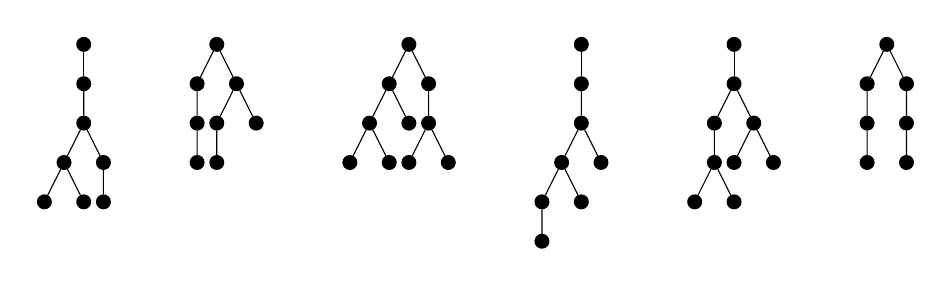
\begin{tikzpicture}[level distance=0.5cm,level/.style={sibling distance=0.5cm}]

    \matrix[column sep=1cm]
    {
      \node[vertex] {}
        child {node[vertex] {}
          child {node[vertex] {}
            child {node[vertex] {}
              child {node[vertex] {}}
              child {node[vertex] {}}
            }
            child {node[vertex] {}
              child {node[vertex] {}}
            }
          }
        };
    &
      \node[vertex] {}
        child {node[vertex] {}
          child {node[vertex] {}
            child {node[vertex] {}}
          }
        }
        child {node[vertex] {}
          child {node[vertex] {}
            child {node[vertex] {}}
          }
          child {node[vertex] {}}
        };
    &
      \node[vertex] {}
        child {node[vertex] {}
          child {node[vertex] {}
            child {node[vertex] {}}
            child {node[vertex] {}}
          }
          child {node[vertex] {}}
        }
        child {node[vertex] {}
          child {node[vertex] {}
            child {node[vertex] {}}
            child {node[vertex] {}}
          }
        };
    &
      \node[vertex] {}
        child {node[vertex] {}
          child {node[vertex] {}
            child {node[vertex] {}
              child {node[vertex] {}
                child {node[vertex] {}}
              }
              child {node[vertex] {}}
            }
            child {node[vertex] {}}
          }
        };
    &
      \node[vertex] {}
        child {node[vertex] {}
          child {node[vertex] {}
            child {node[vertex] {}
              child {node[vertex] {}}
              child {node[vertex] {}}
            }
          }
          child {node[vertex] {}
            child {node[vertex] {}}
            child {node[vertex] {}}
          }
        };
    &
      \node[vertex] {}
        child {node[vertex] {}
          child {node[vertex] {}
            child {node[vertex] {}}
          }
        }
        child {node[vertex] {}
          child {node[vertex] {}
            child {node[vertex] {}}
          }
        };
    \\
    };

  \end{tikzpicture}

\end{figure}

  In this figure we can see that both rules will match on leaf nodes due to the dangling condition. As such the system will need to mark just the leaf nodes as available nodes. It must also unmark nodes that become parent nodes. In $r_1$, the rule converts a leaf node into a parent node but also adds an available node, so the total available nodes increases by zero. On the other hand $r_2$ adds two new nodes so the total available nodes increases by one.

  The figure below shows an example of the system applied to the same grammar with the number of vertices bound $\leq 10$.
  \begin{figure}[!h]
  \centering
  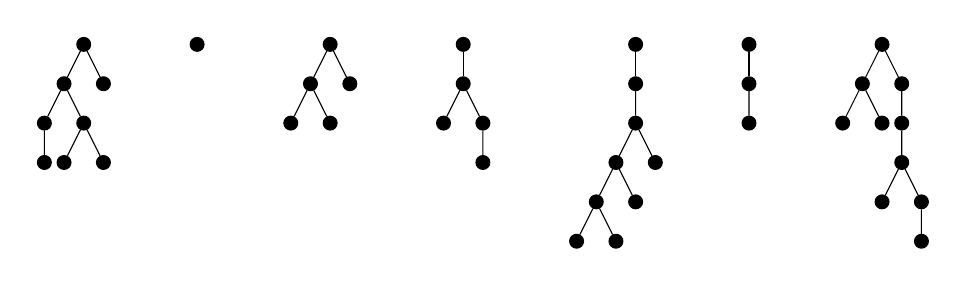
\begin{tikzpicture}[level distance=0.5cm,level/.style={sibling distance=0.5cm}]

    \matrix[column sep=1cm]
    {
      \node[vertex] {}
        child {node[vertex] {}
          child {node[vertex] {}
            child {node[vertex] {}}
          }
          child {node[vertex] {}
            child {node[vertex] {}}
            child {node[vertex] {}}
          }
        }
        child {node[vertex] {}};
    &
      \node[vertex] {};
    &
      \node[vertex] {}
        child {node[vertex] {}
          child {node[vertex] {}}
          child {node[vertex] {}}
        }
        child {node[vertex] {}};
    &
      \node[vertex] {}
        child {node[vertex] {}
          child {node[vertex] {}}
            child {node[vertex] {}
            child {node[vertex] {}}
          }
        };
    &
      \node[vertex] {}
        child {node[vertex] {}
          child {node[vertex] {}
            child {node[vertex] {}
              child {node[vertex] {}
                child {node[vertex] {}}
                child {node[vertex] {}}
              }
              child {node[vertex] {}}
            }
            child {node[vertex] {}}
          }
        };
    &
      \node[vertex] {}
        child {node[vertex] {}
          child {node[vertex] {}}
        };
    &
      \node[vertex] {}
        child {node[vertex] {}
          child {node[vertex] {}}
          child {node[vertex] {}}
        }
        child {node[vertex] {}
          child {node[vertex] {}
            child {node[vertex] {}
              child {node[vertex] {}}
              child {node[vertex] {}
                child {node[vertex] {}}
              }
            }
          }
        };
    \\
    };

  \end{tikzpicture}

\end{figure}

  \subsubsection{Improvement on Ranjan's Approach}

  It is likely that the reason Ranjan's approach happens in two stages is a workaround to GP which has a very simple instruction set. By changing the method keep a sequence of morphisms, we can improve it a bit.

  \begin{itemize}
  \item Let $d$ be a sequence of all isomorphic graph morphisms to $G$ for each rule in the grammar.
  \item Pick a random integer $1 \leq r \leq \#d$ and apply rule $d_r$ to the graph $G$.
  \item Update the sequence $d$
  \item Repeat loop until some condition
  \end{itemize}

  This method is a more general version of Ranjan's approach and there are no restrictions of the grammar. However, the implementation of this method is very expensive to compute since matching morphisms is not trivial.

  Another method is to use what we know about hypergraph languages. Below is a new method that works on hypergraphs. It keeps a sequence of available non-terminals and picks one at random. It then chooses a random rule that can be applied to this location and applies it the the graph. Using a sequence of non-terminals instead of graph morphisms gives a better computational speed since the lookup of non-terminals in a graph is a constant time operation.

  \begin{itemize}
  \item Let $G$ be the start graph. Let $d$ be a sequence of all the non-terminal hyperedges in $G$
  \item Begin loop
  \item Pick a random integer $1 \leq l \leq \#d$.
  \item Get the set of all valid rules on this edge. $r = \{\textrm{All rules $\langle x \to R \rangle$ where $x = lbl_F(d_l)$\}}$
  \item Pick another random integer $1 \leq m \leq \#r$ and apply the rule $r_m$ to the graph $G$.
  \item Remove the non-terminal $d_l$ from $d$ and add all the non-terminals in the replaced graph $R$.
  \item Repeat loop
  \end{itemize}
\bibliography{references}{}
\bibliographystyle{plain}

\end{document}
